\chapter{Gate defined triangular cavities}

In the previous chapter we have found that the best geometries to couple MBS are the ring and the triangular geometries.
The coupling of different pairs is highly asymmetric in the ring geometry, while it is similar in the triangular geometry.
Then, we consider that a triangular trijunction is more reliable when selectively coupling multiple MBS pairs.

In this chapter, we simulate a gate defined triangular cavity and describe how it can be used as a switch coupling different MBS pairs.
The electrostatic potential is found as the solution to Eq. \eqref{} using the finite element solver from Ref. .
In practice, the cavity region in the trijunction is filled with the electrostatic potential, while the nanowires are set to a step like-potential.

\section{Gates configuration}

A trijunction is a complex Majorana device that can be implemented on a 2DEG by selectively depositing electrostatic gates.
It contains two main regions: three nanowires and a semiconducting cavity.
We focus on the design of a gate defined triangular cavity.
We do not consider the electrostatic modeling of the nanowires since one can assume that the electric field in the nanowires is screened by the superconductor.

The gates are placed in a single layer above the 2DEG with a dielectric layer in the middle as shown in Fig. .
Different layer configurations were explored, and a single layer was found to be the best in terms of shape-resolution and voltage range.
The thickness of each layer determines how much the electric field penetrates into the 2DEG.
We consider typical parameters from experiments as described in the inset of Fig. .

\begin{figure}[h!]
\centering
  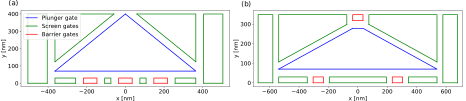
\includegraphics[width=\linewidth]{figures/gate_configurations.pdf}
  \caption{Gate configuration of the two triangular cavities considered. The area is set $A=1200$ $[a^2]$. (a) Triangular cavity with angle $\theta = 0.234 \pi$ with all nanowires at the lower side. (b) Triangular cavity with angle $\theta = 0.125\pi$ with central nanowire at the top side. Spacing between gates is set to $40$ nm. Barrier gates have length $30$ nm and width $70$ nm. Nanowires (not shown) are attached at the ends of the barrier gates.}
  \label{fig:gates}
\end{figure}

Let us consider the two gate configurations shown in Fig. for the cavity region.
There are three kinds of gates:
\begin{enumerate}
\item Plunger gate: Defines and controls the potential inside the triangular cavity region.
\item Screen gates: There are two kinds of screen gates: First, the triangular screen gates deplete the 2DEG around the plunger gate, which contributes to the overall triangular shape. Second, the screen barrier gates between the tunnel gates that keep each nanowire channel separated from the others.
\item Barrier gates: Modulate the coupling between each nanowire and the cavity. They allow to tune the system in the insulating, tunnelling, and strong coupling regimes.
\end{enumerate}

In general terms, to operate the device optimally we require the minimum number of tunable gates while having enough flexibility to connect different MBS pairs.
There are three basic requirements that must be satisfied at all times:
\begin{enumerate}
\item Selectively couple different pairs of MBS via control of barrier gates.
\item Use the triangular screen gates to deplete the area surrounding the plunger gate.
\item There is always a barrier between successive tunnel gates by tuning screen gates.
\end{enumerate}
The first two requirements require us to calibrate the device with focus on varying the minimum number of gate voltages.
The last requirement can be satisfied by choosing a sufficiently large screen barrier.

\section{Device 1}

\begin{figure}[h!]
\centering
  \includegraphics[width=\linewidth]{figures/device_1_potential.pdf}
  \caption{Equipotential lines inside the device for representative parameters of the (a) left and right MBS pair and (b) left and center MBS pair. Colorbar indicates value of equipotential lines. (c) Cut of the potential along the tunnel barriers, i.e. dashed black lines in (a) and (b), taken for a range of plunger gate voltages. Colorbar in (c) indicates the plunger gate voltage.}
  \label{fig:device_1_barriers}
\end{figure}

In this section we describe the operation of the gate configuration shown in Fig. \ref{fig:gates} (a).
Here, special attention to the barrier gates is required since they are close to each other, and the interdependence between them
In Fig.  \ref{fig:device_1_barriers} (a) - (b) one can observe the potential inside the 2DEG for the coupling of each pair.
In contrast to the geometrical model discussed in the previous chapter, the triijunction is defined in a smooth potential landscape.
Therefore, it is not clear if the geometrical dependence that we discussed in Fig. \ref{fig:} will hold.

\subsection{Nanowire channels}

\begin{figure}[h!]
\centering
  \includegraphics[width=\linewidth]{figures/device_1_barriers.pdf}
  \caption{Coupling of (a) left and right MBS pair and (b) left and central MBS pair as a function of the corresponding barrier gates. Plunger gate is tuned around the first resonance. Gate voltages used correspond to those described in Table \ref{table:gate_voltages}.}
  \label{fig:device_1_barriers}
\end{figure}

Operating the left and right tunnel barriers is straightforward since they are far from each other.
Consequently, there is no interdependence between them as can be observed in Fig. \ref{fig:device_1_barriers} (a).
On the other hand, the operation of the central pairs is not symmetric given the mutual influence of successive barrier gates.
In Fig. \ref{fig:device_1_barriers} (b) one can observe that the slope of the potential crossings is not zero indicating cross interaction.

The system can be tuned in the insulating, tunnel, and strong coupling regimes by manipulating the barrier gates.
The blue and orange lines in Fig. indicate the value of the potential at the bottom of the barrier gates with respect to $\mu_0$ and $0$, respectively.
The tunnelling regime starts at the blue line, when the barrier potential crosses $\mu_0$.
In this regime, the coupling is mediated by direct overlap of the MBS wavefunctions.
Therefore, one observes a difference in the tunnelling regime of panels (a) and (b) since in the later the MBS are closer.
The orange lines indicate the start of the strong coupling regime, after which the MBS coupling saturates.

As the barrier potential becomes more positive, there are two new effects:
New crossings caused by resonant cavity levels appear.
On the other hand, for very large barrier gates the screen barrier between them lowers and allows for direct coupling.
The former can be seen clearly in panel (a) as the two crossings in the strong coupling regime.
The later can be seen in the lower right part of panel (b) where the coupling increases due to direct coupling.
Nevertheless, keeping the barrier potential as small as possible makes these effects negligible.

\subsection{Background potential}

\begin{figure}[h!]
\centering
  \includegraphics[width=\linewidth]{figures/device_1_screens.pdf}
  \caption{Coupling of (a) left and right MBS pair and (b) left and central MBS pair as a function of the triangular screen gates. Plunger gate is tuned around the first resonance. Gate voltages used correspond to those described in Table \ref{table:gate_voltages}.}
  \label{fig:device_1_screens}
\end{figure}

In contrast to the purely geometrical model, the triangular cavity can be deformed by tuning the screen gates, and new coupling regimes can be explored.
By increasing the voltage of the screen gates, one confines the electronic density within the triangular cavity.

In Fig. \ref{fig:device_1_screens} one can observe the MBS coupling as a function of the voltages of the two triangular screen gates for each pair.
In panel (a) one observes that the case of the left and right MBS pair is symmetric.
As expected, there is a peak in the coupling when the electronic density is confined to the triangular cavity.

On the other hand, panel (b) shows a new regime for the coupling of the central MBS pairs.
One observes that the coupling of the left central pair increases by increasing the potential in the right triangular screen gate.
Effectively, the cavity becomes smaller, and the coupling increases due to a higher wavefunction overlap.

\subsection{Device operation}

The device is operated as a switch that maximises the coupling between different MBS pairs.
Once a given pair is coupled, four gates are required to change in order to couple a different pair.
Based on the discussion from the previous sections, the set of gate voltages that define the operational point of the device are shown in Table \ref{table:gate_voltages}.
One can observe that 

\begin{table}[h!]
\centering
\begin{tabular}{||c || c c c c c c ||} 
 \hline
& $V_{plunger}$ & $V_{barrier}^L$ & $V_{barrier}^R$ & $V_{barrier}^C$ & $V_{screen}^L$ & $V_{screen}^R$ \\
 \hline\hline
 left-right & 3 & 35 & 35 & -20 & -15 & -15\\ 
 \hline
 left-center & 1 & 35 & -20 & 20 & -15 & 40\\ 
 \hline
 center-right & 1 & -20 & 35 & 20 & 40 & -15\\ 
 \hline
 \hline
\end{tabular}
\caption{Gate voltage configuration used for coupling different MBS pairs. Voltage units are $meV$. Remaining gate voltages are fixed: screen barriers between nanowires $-30$ meV, screen barriers around nanowires $-15$ meV.}
\label{table:gate_voltages}
\end{table}

\section{Device 2}

\begin{figure}[h!]
\centering
  \includegraphics[width=0.7\linewidth]{figures/device_2_potential.pdf}
  \caption{Equipotential lines inside the device for representative parameters of the (a) left and right MBS pair and (b) left and center MBS pair. Colorbar indicates value of equipotential lines. (c) Cut of the potential along the tunnel barriers, i.e. dashed black lines in (a) and (b), taken for a range of plunger gate voltages. Colorbar in (c) indicates the plunger gate voltage.}
  \label{fig:device_2_barriers}
\end{figure}

In this section we describe the operation of the gate configuration shown in Fig. \ref{fig:gates} (b).
In Fig.  \ref{fig:device_2_barriers} (a) - (b) one can observe the potential inside the 2DEG for the coupling of each pair.
While the area in both devices is the same, this device has a smaller angle.
The overall shape resembles a quasi-one dimensional system where resonant trapping is expected.

\subsection{Nanowire channels}

\begin{figure}[h!]
\centering
  \includegraphics[width=\linewidth]{figures/device_2_barriers.pdf}
  \caption{Coupling of (a) left and right MBS pair and (b) left and central MBS pair as a function of the corresponding barrier gates. Plunger gate is tuned around the first resonance. Gate voltages used correspond to those described in Table \ref{table:gate_voltages}.}
  \label{fig:device_2_barriers}
\end{figure}

In contrast to the previous device, all barrier gates remain well separated from each other.
Therefore, in Fig. \ref{fig:device_2_barriers} one observes that there is no interdependence of barrier gates.
However, the system behaves effectively as a quasi-one dimensional cavity.
Consequently, the coupling in the tunnelling regime is larger due to an increase in the wavefunction overlap.

In the strong coupling regime there is a large difference between the coupling of the different pairs.
One can observe that panel (a) is similar to the previous case.
On the other hand, panel (b) shows a very different behaviour that reflects the new structure of the cavity.
This effect was not present in the purely geometric model, which suggest that it does not hold for gate defined cavities.

\subsection{Potential background}

\begin{figure}[h!]
\centering
  \includegraphics[width=\linewidth]{figures/device_2_screens.pdf}
  \caption{Coupling of (a) left and right MBS pair and (b) left and central MBS pair as a function of the triangular screen gates. Plunger gate is tuned around the first resonance. Gate voltages used correspond to those described in Table \ref{table:gate_voltages}.}
  \label{fig:device_2_screens}
\end{figure}

In this device the position of the barrier gates is highly dependent on the surrounding screen gates as can be observed in Fig. \ref{fig:device_2_barriers}.
Therefore, it is not possible to strongly deform triangular cavity without disconnecting the nanowires.

Similar as before, in Fig. \ref{fig:device_2_screens} (a) one observes that there is a region where the MBS coupling for the left and right MBS pair has a maximum.
This region corresponds to the electronic density concentrated under the plunger gate.
Interestingly, the magnitude of the coupling is similar to the previous device.

The coupling of the central pairs as a function of the screen gates can be observed in panel (b).
One can observe that there's a region where a maximum develops, but it remains smaller than the coupling of the left and right MBS pair.
Furthermore, the coupling vanishes if the right triangular screen gate becomes very negative.
This indicates that the barrier gate has been displaced from its position, and the central nanowire disconnects from the cavity.

If the screen gates are not tuned correctly, the coupling vanishes.
If the screen gates are too negative, the area under the plunger gate is depleted, and the MBS cannot couple.
Similarly, if is not negative enough, the electron density is extended over a rectangular region and the coupling becomes very small.

\subsection{Device operation}

This device can be used as a switch to couple different MBS pairs selectively.
However, the magnitude of the coupling is highly asymmetric between pairs.
Consequently, 

\begin{table}[h!]
\centering
\begin{tabular}{||c || c c c c c c ||} 
 \hline
& $V_{plunger}$ & $V_{barrier}^L$ & $V_{barrier}^R$ & $V_{barrier}^C$ & $V_{screen}^L$ & $V_{screen}^R$ \\
 \hline\hline
 left-right & 6 & 17 & 17 & -20 & -15 & -15\\ 
 \hline
 left-center & 6.7 & 17 & -20 & 17 & -10 & -20\\ 
 \hline
 center-right & 6.7 & -20 & 17 & 17 & -20 & -10\\ 
 \hline
 \hline
\end{tabular}
\caption{Gate voltage configuration used for coupling different MBS pairs. Voltage units are $meV$. Remaining gate voltages are fixed: screen barriers between nanowires $-30$ meV, screen barriers around nanowires $-15$ meV.}
\label{table:gate_voltages}
\end{table}


\section{Devices comparison}

\begin{figure}[h!]
\centering
  \includegraphics[width=0.8\linewidth]{figures/device_couplings.pdf}
  \caption{}
  \label{fig:device_2_screens}
\end{figure}

